\documentclass[9pt,letterpaper,twoside]{article}

\usepackage[authoryear]{natbib}
\usepackage{times} 
\usepackage{amsmath,amsfonts}
\usepackage{graphicx}
\usepackage{setspace}
\usepackage{indentfirst}
\usepackage{color}
\usepackage[paper=letterpaper]{geometry}
\usepackage{fontspec}
\setmainfont[Mapping=text-tex]{Calibri}

% revise margins
\setlength{\headheight}{0.25in}
\setlength{\headsep}{-0.25in}
\setlength{\topmargin}{0.0in}
\setlength{\textheight}{9in}
\setlength{\footskip}{0.5in}
\setlength{\oddsidemargin}{0in}
\setlength{\evensidemargin}{0in}
\setlength{\textwidth}{6.5in}
\setlength{\rightskip}{0pt plus 1fil} % makes ragged right


% headings
\usepackage{fancyhdr}
\pagestyle{fancy}
\fancyfoot{}
\fancyfoot[C]{K. W. Broman}
\fancyfoot[RO, LE]{\textbf{\thepage\ SI}}
\fancyhead{}
\renewcommand{\headrulewidth}{0pt}
\renewcommand{\footrulewidth}{0pt}

\begin{document}
\thispagestyle{empty}


\vspace*{8mm}
\begin{center}

\textbf{\Large Genotype probabilities at intermediate generations\\[18pt]
in the construction of recombinant inbred lines}
 
\bigskip \bigskip
 
\bigskip \bigskip
 
\textbf{\Large SUPPLEMENT}

\bigskip \bigskip
\bigskip \bigskip
 
 
{\large Karl W. Broman\\[12pt]
Department of Biostatistics and Medical Informatics, \\[12pt]
University of Wisconsin--Madison, Madison, Wisconsin 53706 }
\end{center}


\vfill

\hfill 
{\footnotesize 14 September 2011}

\newpage

{
\centering
\includegraphics[width=\textwidth]{Figs/onelocus_fig.eps}

\bigskip
\textbf{Figure S1} {\color{white} n} One-locus genotype probabilities for 
a random individual on the autosome \textbf{(A)},  the female on the X
chromosome \textbf{(B)}, and the male on the X chromosome \textbf{(C)}, at
generation $\text{F}_k$ in the production of four-way RIL by sibling
mating, as a function of $k$.
}


\clearpage


{
\centering
\includegraphics[width=\textwidth]{Figs/riXfig.eps}

\bigskip
\textbf{Figure S2} {\color{white} n} The X chromosome in the generation of two-way (A), four-way
(B), and eight-way (C) RIL by sibling mating.
}

\clearpage

{
\centering
\includegraphics[width=\textwidth]{Figs/happrob_fig.eps}

\bigskip
\textbf{Figure S3} {\color{white} n} Two-locus haplotype probabilities, as a function of
recombination fraction, for 
a random autosome haplotype (left column),  a random X
chromosome haplotype
from the female (middle column), and the male X chromosome haplotype
(right column)  at
generation $\text{F}_k$ in the production of four-way RIL by sibling
mating, with the individual curves corresponding to different values
of $k$.
}






\newpage


\noindent \textbf{Table S1 {\color{white} n} Recursion matrix for calculating
two-locus autosomal haplotype probabilities in the generation of four-way RIL by
sibling mating}

\bigskip

{\setstretch{2.0}
KWBinsert:Tables/hap_autosome_tm_supp_table.tex
}

\newpage

\noindent \textbf{Table S2 {\color{white} n} Starting states for calculating
two-locus autosomal haplotype probabilities in the generation of four-way RIL by
sibling mating}

{\setstretch{2.0}
KWBinsert:Tables/hap_autosome_start_supp_table.tex
}

\bigskip

\newpage

\noindent \textbf{Table S3 {\color{white} n} Transition matrix for two loci
in the generation of two-way RIL by selfing}

\bigskip

{\setstretch{1.3}
KWBinsert:Tables/selfing_supp_table.tex
}

\newpage


\noindent \textbf{Table S4 {\color{white} n} Transition matrix for one autosomal locus
in the generation of four-way RIL by sibling mating}

\bigskip

{\setstretch{1.5}
KWBinsert:Tables/onelocus_autosome_tm_supp_table.tex
}

\newpage


\noindent \textbf{Table S5 {\color{white} n} Probabilities for the genotypes of the 
pair of individuals at a single autosomal locus, at generation $\text{F}_{\boldsymbol{k}}$
in the formation of four-way RIL by sibling mating}

\bigskip

{\setstretch{1.7}
KWBinsert:Tables/onelocus_autosome_results_supp_table.tex
}

\newpage


\noindent \textbf{Table S6 {\color{white} n} Transition matrix for one X chromosome
locus in the generation of four-way RIL by sibling mating}

\bigskip

{\setstretch{1.5}
KWBinsert:Tables/onelocus_Xchr_tm_supp_table.tex
}

\newpage

\noindent \textbf{Table S7 {\color{white} n} Probabilities for the genotypes of the 
pair of individuals at a single X chromosome locus, at generation $\text{F}_{\boldsymbol{k}}$
in the formation of four-way RIL by sibling mating}

\bigskip

{\setstretch{1.7}
KWBinsert:Tables/onelocus_Xchr_results_supp_table.tex
}

\newpage


\noindent \textbf{Table S8 {\color{white} n} Recursion matrix for calculating
two-locus X chromosome haplotype probabilities in the generation of four-way RIL by
sibling mating}

\bigskip

{\setstretch{2.0}
KWBinsert:Tables/hap_Xchr_tm_supp_table.tex
}

\newpage

\noindent \textbf{Table S9 {\color{white} n} Starting states for calculating
two-locus X chromosome haplotype probabilities in the generation of four-way RIL by
sibling mating}

\bigskip

{\setstretch{2.0}
KWBinsert:Tables/hap_Xchr_start_supp_table.tex
}

\newpage

\noindent \textbf{Table S10 {\color{white} n} Transpose of the recursion matrix for
calculating probabilities of two-locus autosomal diplotypes of the form $\boldsymbol{\boldsymbol{AA|AA}}$,
in the generation of four-way RIL by sibling mating.  Only the
non-zero entries are shown}

\bigskip

{\setstretch{2.0}
KWBinsert:Tables/twolociA4_AA_AA_supp_table.tex
}

\newpage

\noindent \textbf{Table S11 {\color{white} n} Starting states for the calculation of
probabilities of two-locus autosomal diplotypes of the form $\boldsymbol{AA|AA}$,
in the generation of four-way RIL by sibling mating}

\bigskip

{\setstretch{2.0}
KWBinsert:Tables/twolociA4_AA_AA_start_supp_table.tex
}

\newpage

\noindent \textbf{Table S12 {\color{white} n} Transpose of the recursion matrix for
calculating probabilities of two-locus autosomal diplotypes of the form $\boldsymbol{AA|AB}$,
in the generation of four-way RIL by sibling mating}

\bigskip

{\setstretch{2.0}
KWBinsert:Tables/twolociA4_AA_AB_supp_table.tex
}

\newpage

\noindent \textbf{Table S13 {\color{white} n} Starting states for the calculation of
probabilities of two-locus autosomal diplotypes of the form $\boldsymbol{AA|AB}$,
in the generation of four-way RIL by sibling mating}

\bigskip

{\setstretch{2.0}
KWBinsert:Tables/twolociA4_AA_AB_start_supp_table.tex
}

\newpage

\noindent \textbf{Table S14 {\color{white} n} Transpose of the recursion matrix for
calculating probabilities of two-locus autosomal diplotypes of the form $\boldsymbol{AA|BB}$,
in the generation of four-way RIL by sibling mating}

\bigskip

{\setstretch{2.0}
KWBinsert:Tables/twolociA4_AA_BB_supp_table.tex
}


\newpage

\noindent \textbf{Table S15 {\color{white} n} Starting states for the calculation of
probabilities of two-locus autosomal diplotypes of the form $\boldsymbol{AA|BB}$, 
in the generation of four-way RIL by sibling mating}

\bigskip

{\setstretch{2.0}
KWBinsert:Tables/twolociA4_AA_BB_start_supp_table.tex
}

\newpage

\noindent \textbf{Table S16 {\color{white} n} Transpose of the recursion matrix for
calculating probabilities of the two-locus X chromosome female diplotype of the form $\boldsymbol{AA|AA}$,
in the generation of four-way RIL by sibling mating}

\bigskip

{\setstretch{2.0}
KWBinsert:Tables/twolociX4_female_AA_AA_supp_table.tex
}
\newpage

\noindent \textbf{Table S17 {\color{white} n} Starting states for the calculation of
probabilities of the two-locus X chromosome female diplotype of the form $\boldsymbol{AA|AA}$, 
in the generation of four-way RIL by sibling mating}

\bigskip

{\setstretch{2.0}
KWBinsert:Tables/twolociX4_female_AA_AA_start_supp_table.tex
}

\newpage

\noindent \textbf{Table S18 {\color{white} n} Transpose of the recursion matrix for
calculating probabilities of the two-locus X chromosome female diplotype of the form $\boldsymbol{AA|AB}$, 
in the generation of four-way RIL by sibling mating}

\bigskip

{\setstretch{2.0}
KWBinsert:Tables/twolociX4_female_AA_AB_supp_table.tex
}

\newpage

\noindent \textbf{Table S19 {\color{white} n} Starting states for the calculation of
probabilities of the two-locus X chromosome female diplotype of the form $\boldsymbol{AA|AB}$,
in the generation of four-way RIL by sibling mating}

\bigskip

{\setstretch{2.0}
KWBinsert:Tables/twolociX4_female_AA_AB_start_supp_table.tex
}

\newpage

\noindent \textbf{Table S20 {\color{white} n} Transpose of the recursion matrix for
calculating probabilities of the two-locus X chromosome female diplotype of the form $\boldsymbol{AA|BB}$,
in the generation of four-way RIL by sibling mating}

\bigskip

{\setstretch{2.0}
KWBinsert:Tables/twolociX4_female_AA_BB_supp_table.tex
}

\newpage

\noindent \textbf{Table S21 {\color{white} n} Starting states for the calculation of
probabilities of the two-locus X chromosome female diplotype of the form $\boldsymbol{AA|BB}$,
in the generation four-way RIL by sibling mating}

\bigskip

{\setstretch{2.0}
KWBinsert:Tables/twolociX4_female_AA_BB_start_supp_table.tex
}

\newpage

\noindent \textbf{Table S22 {\color{white} n} Prescription for the calculation of two-locus
autosomal diplotype probabilities at intermediate generations in the
construction of 8-way RIL, from the corresponding probabilities for
4-way RIL}

\bigskip

{\setstretch{1.6}
KWBinsert:Tables/statesA8_supp_table.tex
}
\newpage

\noindent \textbf{Table S23 {\color{white} n} Prescription for the calculation of two-locus X
chromosome female diplotype probabilities at intermediate generations
in the construction of 8-way RIL, from the corresponding probabilities
for 4-way RIL. Only the states with non-zero probability are shown.}

\bigskip

{\setstretch{1.6}
KWBinsert:Tables/statesX8_supp_table.tex
}


\end{document}
